%!TEX root = ../dissertation.tex

% \begin{savequote}[85mm]
% 	\itshape The basic theorem of interdisciplinary research states: \\
% 	\itshape physicists not only know everything; they know everything better \\
% 	\itshape This theorem is wrong; it is valid only for \\
% 	\itshape computational statistical physicists like me.\cite{Stauffer_2004}
% 	\qauthor{---Dietrich Stauffer}
% \end{savequote}

\chapter{Materials \textit{\&} Methods}
\label{chap:02}

\Lettrine{Computational chemistry} was first coined by Frank Westheimer at a conference in 1966 to refer to Allinger's work on molecular mechanics,\cite{Lipkowitz_2000} separating it from other studies that would fall under the \textit{theoretical chemistry} category at that time. Nowadays, the term is broader and considers far more techniques. In fact, under the modern definition earlier works would be considered \textit{computational chemistry}; albeit analog ones. In 1930, Kettering and more researchers in General Motors, built ball-and-spring models for several molecules and correlated their vibration modes with their Raman spectra. This work, titled \textit{A representation of the dynamic properties of molecules by mechanical models},\cite{kettering1930} could be considered one of the first molecular modeling studies.

\section{Origins of molecular modeling}
% \addcontentsline{toc}{section}{Origins of molecular modeling}
The birth of theoretical chemistry, from a quantum chemistry perspective, can be pinpointed with the description of the Schrödinger equations in 1925--1926.\cite{schrodinger} The first application of quantum mechanics came a year later, in 1927, with the publication of Burrau's studies\cite{burrau1927} on $H_{2}^{+}$ and Heitler and London calculations\cite{heitlerlondon} on $H_{2}$. The field began to grow rapidly (Teller,\cite{teller1930hydrogen} Mulliken,\cite{mulliken} Born,\cite{born} Oppenheimer,\cite{Oppenheimer} Pauling,\cite{pauling} Hückel,\cite{huckel} Hartree,\cite{hartree} Fock\cite{fock}\ldots) and computational implementations of the new theoretical framework started to be feasible after the advances in computer technology during the late 40s.\cite{chistory1940} In the 50s and 60s, several milestone papers were published, making for the first documented computational chemistry calculations.\cite{bolcer2007,ccl} Also, non-quantum, classical approaches stemming from theoretical physics started to emerge, although not strictly dealing with chemistry problems.\cite{Alder1959,Gibson1960,Rahman1964}

By the 70s, several journals had appeared to target computational chemistry and the first quantum chemistry packages began to be distributed (including the first version of the now ubiquitous Gaussian\cite{gaussian}). The available hardware back then only allowed for \textit{ab initio}\footnote{ A model is said to be \textit{ab initio} when it only considers the resolution of the first principle equations (Schrödinger's), without support from experimental observations. Empirically derived models do take these observations into account, very often as a workaround to avoid solving the full equation system. When the two approaches are combined, those are semi-empirical methods.  } calculations of molecules as big as naphthalene and azulene (18 atoms). In those same years, molecular mechanics methods became more popular, especially with the contributions by Lifson's CFF,\cite{lifson1968consistent,hagler1974energy,niketic1977lecture} Allinger's MM series,\cite{allinger1973,allinger1977} Scheraga's ECEPP potentials,\cite{momany1975energy,nemethy1983energy} Karplus’ CHARMM,\cite{brooks1983} van Gunsteren's GROMOS\cite{van1987groningen} and others, proving the power of empirical parameterization. By the 80s, Computer Assisted Molecular Design (CAMD) was the new hype that would revolutionize the pharmaceutical industry,\cite{fortune1981} and by the 90s it was clear that computational chemistry was broader than quantum chemistry. In the preface of \textit{Reviews in Computational Chemistry Volume I},\cite{lipkovitz1990} editors acknowledge that:

\begin{quote}
	"[...] we do not view the terms theoretical chemistry and computational chemistry as synonymous. Computational chemistry sometimes involves application of computerized algorithms from quantum theory, but computational chemistry is certainly more than quantum chemistry [...]. Molecular mechanics, molecular dynamics, computer graphics, molecular modeling, and computer-assisted molecular design are other important aspects of computational chemistry [...]".
\end{quote}

Nowadays, molecular modeling encompasses techniques and strategies beyond what is traditionally considered computational chemistry (this is, quantum and molecular mechanics, mainly). With the current popularity of more expressive languages, it will be possible to devise new algorithms and protocols in less time. Additionally, it can be argued that recent advances do not only come from developing new methods, but also from reapplying the existing ones under new computational architectures, both in terms of hardware and software. For example, parallelizable code and, in particular, GPU-acceleration, have taken the performance of Molecular Mechanics methods to the next level.\footnote{Quantum Mechanics software is also starting to use GPU-accelerated code, but the support is still limited (see \autoref[appendix]{chap:appendix-a}).}

The following pages will introduce the major families of software approaches in computational chemistry and molecular modeling. They will be listed in two major groups depending on the focus (energy description or conformational sampling), and in descending order of level of theory,\footnote{An estimation of the complexity of the theory supporting the method, that while arbitrary, gives a quick understanding of the intricacies involved. Higher theory levels usually refer to highly accurate, computationally demanding methods that rely on complex mathematical models. Lower theory levels, on the contrary, refer to less accurate and computationally cheap methods relying on simpler models.} which, in practice, means going from high-accuracy to lower-accuracy methods. Finally, an overview on optimization methods will depict the relationships between energy description and space sampling in the context of molecular modeling.

% [FIGURE: Timeline of molecular modeling milestones] TODO!

\section{Energy description}
% \addcontentsline{toc}{subsection}{Methods focused on energy description}
\subsection{Quantum Mechanics (QM)}
% \addcontentsline{toc}{subsubsection}{Quantum Mechanics (QM)}
\label{section:qm}

The main idea behind quantum chemistry is that molecules and, by extension, all ordinary matter, can be viewed as composed only of positively charged nuclei and negatively charged electrons. Mathematically, this can be expressed with the time-independent Schrödinger equation:

\begin{align}
	H \Psi =E \Psi =T_{n}+T_{e}+V_{ne}+V_{ee}+V_{nn} \\ \tag{Time-independent Schrödinger's equation}
\end{align}

, where $H$ is the Hamiltonian operator, $E$ is the total energy of the system, $T_{n}$ and $T_{e}$ are the kinetic energies of nuclei and electrons, respectively, and $V_{ne}$, $V_{ee}$ and $V_{nn}$ are the potential energy between nuclei and electrons, electrons against each other, and nuclei against each other, respectively. Solving this equation for any system would mean seeking the eigenfunctions and eigenvalues of that Hamiltonian.

The details of such resolution are out of the scope of this thesis, but some comments can be made about its practical effects. Since only one-particle and two-particle systems can be solved analytically, numerical methods are employed to approximate the solution for systems of 3 or more particles: the many-body problem. While not analytical, the same methods can be applied iteratively to any given precision; the only restraints are computational and time resources. As a result, some approximations have been developed over the years to simplify the equation solving process without much accuracy loss.

The first approximation to appear was the Born-Oppenheimer approximation. It relies on the big mass difference between nuclei and electrons. In hydrogen, the monoprotonic nucleus is already 1800 times heavier than the electron; for uranium, the nucleus/electron mass ratio goes up to 430,000. This leads to consider that, given the enormous mass difference, electrons and nuclei move in different time-scales: if the nucleus moves, the electrons would follow \textit{instantaneously}. This means that the nucleus can be considered stationary for electronic timescales, and appear as parameters in the equation, greatly simplifying its solution.

Even with uncoupled motions, the dynamics of electrons are complex and require advanced computational methods. A significant simplification would be to treat electrons as independent from each other by introducing an \textit{independent-particle} model, either by neglecting all interactions altogether, or, even better, by introducing an average interaction factor. These approximations are collected under the Hartree-Fock (HF) theory. In HF methods, electronic interactions are not explicitly described, but with a large basis set 99$\%$  of the energy can be described by the HF wave function. The difference between the energy predicted by (Restricted) HF calculations and the real energy is called \textit{electronic correlation}, which in certain chemical phenomena is key to obtaining accurate predictions. As a result, three main strategies have been developed to calculate it explicitly: Configuration Interaction (CI), Many-Body Perturbation Theory (MBPT) and Coupled Cluster (CC).

Evidently, these methods involve extra computational complexity, so in some cases, more aggressive approximations have been applied. This is the case of semi-empirical methods, which instead of trying to resolve some of the most complex integrals, resort to experimental parameterization of the results. While it is true that this leads to less accurate results, they are way faster and, with sensible parameters, the difference can be neglected depending on the study at hand.

HF theory is not the only applicable approximation to simplify the many-electron problem. In a way, Density Functional Theory (DFT) can be seen as a more efficient strategy to tackle the challenge. DFT is based on the Hohenberg and Kohn proof, which suggests that the ground state electronic energy can be determined completely by the electron density. In practice, it offers a computational cost similar to HF theory, but with the possibility of providing more accurate results\footnote{They need a good exchange-correlation functional, though, which can only be obtained exactly for the free electron gas; for other cases, approximations must be employed, like local-density (LDA), local spin-density (LSDA) or generalized gradient (GGA, meta-GGA) approaches.} and is widely used nowadays.

All these methods are applied to solve the time-independent Schrödinger equation; this is, to obtain the energy of a system with given coordinates. If the dynamics of the system (i.e. evolution along time) must be studied, the time-dependent equation must be solved, which involves highly complex calculations to obtain reasonable accuracy. With current resources, only di- and triatomic species can be simulated using this approach. Additional atoms would need to be frozen or treated classically.

A workaround would involve a semi-classical approach. In Ab Initio Molecular Dynamics (AIMD), electrons are treated quantum-mechanically, and nuclei, classically (Born-Oppenheimer Molecular Dynamics, BOMD). At each time step, a converged wave function is obtained and the corresponding nuclear gradients are used to propagate the time-evolution. However, for accurate results, one must resort to tightly converged wave functions (in BOMD) or very small timesteps (in Car-Parrinello Molecular Dynamics, CPMD).

\subsection{Force fields: Molecular Mechanics, Molecular Dynamics and Metadynamics}
% \addcontentsline{toc}{subsubsection}{Force fields: Molecular mechanic, Molecular dynamics and Metadynamics}
\label{section:mm-md}
Depending on the phenomena under study, explicit consideration of electrons is not always necessary. If that's the case, the Schrödinger equation can be bypassed and the electronic energy can be written as a parametric function of the nuclear coordinates. Those parameters are fitted to reproduce either experimental measurements or results obtained with higher levels of theory (i.e. QM). The set of parameters needed to write the set of equations is called \textit{force field}, and the theory behind this strategy is called \textit{Molecular Mechanics} (MM). Given the size of nuclei, these can be treated classically with Newton's second law with sufficient accuracy, resulting in equations much simpler than their QM counterpart, which allow faster computations and, as a result, dealing with larger systems (tens of thousands of atoms). Neglecting the existence of electrons has some consequences, though: bonding information is lost and must be provided explicitly, rather than being an inherent result of the equation.

In MM, molecules are described by a \textit{ball and spring} model: atoms are abstracted as spheres of given radius and \textit{softness}, and bonds have length and \textit{stiffness}. In such an ensemble, the potential energy of the system can be described as the sum of several components: stretching, bending, torsions, non-bonding interactions (usually, Van der Waals and Coulomb), and a cross-term of the first three.

 \begin{align}
	E_{FF}=E_{stretching}+E_{bending}+E_{torsional}+E_{non-bonding}+E_{cross} \\ \tag{Force field energy}
\end{align}

If each of the terms can be expressed as a function of the coordinates for the involved atoms, the potential energy can be obtained, and geometries and relative energies can be calculated by optimization. Thus, all that remains is to obtain the parameters for each type of interaction involved in the system under study. Fortunately, most molecules can be described as a composition of a small set of functional subunits or groups, the properties of which rarely change. For example, all \texttt{C=O} bonds are around 1.22 Å long. Instead of having to parameterize each type of atom and bond for each type of molecule, these similarities allow to construct set of parameters with reasonable easiness, in principle.

As opposed to QM, these equations can be solved efficiently enough to consider time-dependent analysis. If one takes the force field equations and calculates the resulting forces and velocities, the position of the atoms can be figured out with high accuracy if the timestep is small enough (i.e. in the same order of magnitude as the smallest perturbation studied: hydrogen vibration, in the order of femtoseconds). This strategy gives rise to a field called Molecular Dynamics, which allows to study the behavior of molecules along time. Modern computer architectures allow to resolve each timestep around 10\textsuperscript{8} times daily! Processes involving seconds in real-life can be calculated within a month.

Gaining access to such magnitudes allows to calculate properties not available in other higher levels of theory: conformational changes, binding pathways, or thermodynamic magnitudes such as free energy. However, in those calculations the potential energy surface (PES) must be well-sampled. Several methods account for this issue, such as metadynamics (MTD), umbrella sampling or adaptively-biased MD. In the case of MTD, the system is assumed to be describable by a few collective variables or reaction coordinates, which are then explored in such a way that revisiting sampled states is discouraged.

\subsection{QM/MM}
% \addcontentsline{toc}{subsubsection}{QM/MM}
\label{section:qmmm}

Dealing with big systems (more than 300-500 atoms) with QM techniques is not feasible due to computational restraints. In some cases, though, only a subset of the system actually needs explicit consideration of the electrons. One strategy would consist of pruning the nonimportant parts, replacing them by smaller functional units which would keep the system's \textit{chemical identity}.

In other studies, like enzyme reactivity, the nonreactive part of the enzyme is assumed to be important in keeping the active site conformation, and as such, cannot be pruned out. While some authors do model enzyme reactivity with a prune-and-freeze strategy (the \textit{quantum chemical cluster}\cite{siegbahn2009recent}), a large part of the research community prefers to consider the whole protein in the calculation. This can be approached with QM/MM methods, in which the reactive atoms and its immediate surroundings are studied with QM, while the rest of the system is treated classically. The energy of the system is then calculated as a sum of the QM energy, the MM energy and the interaction between both.


\begin{align}
	E_{total}=E_{QM}+E_{MM}+E_{QM/MM} \\ \tag{QM/MM energy}
\end{align}


The independent QM and MM terms can be calculated straightforwardly as explained before, but deciding on how to calculate the interaction is not as intuitive. In general, three strategies can be applied: (1) mechanical embedding, which only considers bonded and steric effects; (2) electrostatic embedding, which also considers the electric field of the MM part; and (3) polarizable embedding, which adds polarizabilities between the QM and MM parts. Even in the simplest case, mechanical embedding, technical difficulties may arise if a bond is cleaved by the QM/MM partitioning, which would require balancing the unpaired electrons in the QM part by adding a \textit{link} atom invisible to the MM part. Similarly, the dangling bond in the MM part must be dealt somehow, normally adding the needed stretching, bending and torsional terms.

Mixing methods of different level theories for a single system is generalized in the ONIOM approach, which assumes additivity of the different \textit{layers}. If two layers are considered, it classifies the system in \textit{model} (the subset of the system which is dealt with a higher level of theory) and \textit{real} (the full model, including the \textit{model} subset). The \textit{model layer} is calculated both with the higher level of theory (usually QM) and the lower one (usually a force field), while the real layer is only calculated with the lower level of theory. Then, the energy is given as:

\begin{align}
  E_{ONIOM}=E_{high}^{real}=E_{high}^{model}-E_{low}^{model}+E_{low}^{real} \\ \tag{ONIOM energy}
\end{align}


Another intrinsic problem to QM/MM methods is the sampling. As the contribution of the MM part to the QM/MM energy is larger than the QM due to the number of atoms involved (around 100 in QM or 1,000-10,000 in MM), reported energy will be very sensitive to even small changes in the MM layer. As a result, when an energy profile must be calculated, the MM part is kept rigid during the whole process, which requires a carefully chosen initial structure to begin with. This usually involves a protocol where a long MD run is performed to obtain a representative snapshot of the simulation.

\subsection{Coarse-grained modeling}

Coarse-grained models constitute an additional simplification level in the diverse representations of molecular models, including proteins,\cite{Kmiecik_2016,Ing_lfsson_2013} nucleic acids,\cite{Boniecki_2015,Potoyan_2012} or lipid membranes.\cite{Baron_2007} Instead of individually describing each atom in the system, they group related atoms together in a single entity. These groups, sometimes called \textit{pseudoatoms}, can have several levels of granularity depending on the system scale. For example, simulating the dynamics of a viral capsid might need monomer-level granularity,\cite{Hagan_2016} while trying to simulate a full cell might involve full organelles being represented individually.\cite{pivkin2008accurate}


% [Figure: ONIOM scheme] % TODO!

\section{Conformational sampling}

Even with the latest advances in computer architecture and software improvements to make the most out of it, some potential energy surfaces are too vast and complex to be explored efficiently with molecular dynamics, let alone quantum dynamics. While this might not apply in the next decade, techniques that take educated shortcuts to traverse broad conformational spaces are still necessary. This is particularly true in large molecules such as proteins, where structural fluctuations occur at very different time scales and amplitudes: local motions take place are fast and short (10\textsuperscript{-15} to 10\textsuperscript{-1}s, 0.01-5 \AA), and collective motions are slow and long (10\textsuperscript{-9} to 1s, 1-10 \AA).

\subsection{Normal Modes Analysis}

In Normal Modes Analysis (NMA), slow, collective motions of a molecular structure can be approximated through the composition of its independent (normal) harmonic oscillations (modes). The NMA approach is parallel to MM in its theoretical support, meaning that bonds are replaced by \textit{springs} or harmonic oscillators. As a result, the mathematical treatment consists of finding the eigenvalue of each coupled oscillator, which is simple enough to be calculated efficiently for thousands of atoms. In fact, there is no obligation to treat each atom and bond independently, as nearby atoms can be grouped together in a new body to reduce the needed number of oscillators (coarse-grained NMA). All these approximations allow dynamic insights on the movements of a macromolecule without the technical limitations of MD, which require long runs to observe slow motions. Since NMA does not consider time at all and only requires an initial structure on which to compute the normal modes, the vibrations obtained only apply to that particular conformation. In other words, only the local potential energy wells are explored, which can provide a short-sighted analysis if no other conformations are assessed.

\subsection{Recognition processes}

Recognition processes involve large conformational changes and are key in research areas such as drug development or metabolic studies. Docking techniques were developed to describe feasible binding modes of small molecules (ligands) within a bigger macromolecule (the host, which is normally a protein). To do that, potential binding pockets in the host are explored explosively by placing the ligand in random orientations and positions (rigid body transformations), contemplating some internal flexibility if necessary (through torsions in the small molecule or rotamer exchange for the side chains in the protein), and finally assessing their non-bonding interactions. Since the spatial landscape needs to be explored efficiently, with thousands of attempts before finding a good pose, the energy representation is often cruder than in higher levels of theory in honor of speed and efficiency: the scoring function. While in principle it could use full molecular dynamics simulations,\cite{Soderhjelm_Tribello_Parrinello_2012,devivo2017} most popular approaches resort to simplifications, like knowledge-based parameters obtained out of structural databases\cite{neudert2011dsx} or empirical evidences.\cite{morris1998automated,baxter1998flexible,korb2009empirical} Other approaches resort to shape complementarity between the Van der Waals surfaces of the involved molecules\cite{venkatachalam2003ligandfit,gabb1997modelling,shoichet1992molecular} or, more recently, to Artificial Intelligence (AI) deep learning techniques.\cite{khamis2015machine}

Docking techniques can also involve other type of molecules, like protein-protein or protein-nucleic acid studies. In this variant, more approximations are needed due to the broader conformational space involved, like only considering rigid-body transformations.

\section{Beyond cartesian coordinates: navigating the chemical space}

Of all the techniques detailed until know, only QM studies allow topology changes like bond breaking or creation. This is, when dealing with MM, NMA or docking, most approaches will assume that the starting set of atoms and their connectivity will be the same during the whole simulation. As a result, to assess different variants of the same compound one must run the same protocol separately for each variant.

The most popular technique employing this strategy is virtual screening, which essentially performs docking calculations for massive datasets of drug-like compounds. In most implementations, the database must be built beforehand and the chemical space is only explored by trying different entries in the dataset. This is, no algorithmic modification of the structure is done during the simulation. With big enough datasets, sampling should not be a problem, but some studies point out that the chemical space explored this way is very limited.\cite{virshup2013stochastic}

Some software projects do attempt to explore the chemical space algorithmically,\cite{oprea2001chemography,bon2010bioactivity,larsson2007chemgps,Goodnow_2016,Reymond_2015,Chari_2015,Maggiora_2014,Naveja_2017} but they still struggle to find mainstream usage in the pharma industry. The implemented approaches often resort to chemical synthesis guidelines like CLICK chemistry\cite{durrant2009} or graph abstractions.\cite{andersen2014} This can be useful in docking calculations that wish to account for some chemical variability in the ligands assessed or rational design of potential inhibitors.

Since protein-ligand docking studies involve at least two molecules, it makes sense to investigate chemical variability in the host. While the theoretical chemical space available in proteins is huge due to the number of atoms alone, fortunately is more constrained: all proteins are chains of the same 20 residues or amino acids. Hence, assessing possible variations \textit{only} involve changing one particular residue for another of the remaining nineteen. It seems simple at first, but the possible variations explode exponentially with chain length, which means that even for small peptides of around 30 residues it results in an unfathomable number: $ 30^{20} $ or around $ 3.5·10^{29} $ (see fig. \ref{fig:chemicalspace}). Subsequently, only a few positions are studied and the variations applied are somehow rational and studied beforehand. Some tools exist to evaluate the potential consequences of a mutation in a protein,\cite{kumar2009predicting,quan2016strum,fariselli2015inps,dehouck2011popmusic} which can help discard destabilizing changes before doing more intense computations. After all, a single change in a key residue can alter the final structure dramatically.\cite{kumar2006protherm}

\begin{figure}[H]
	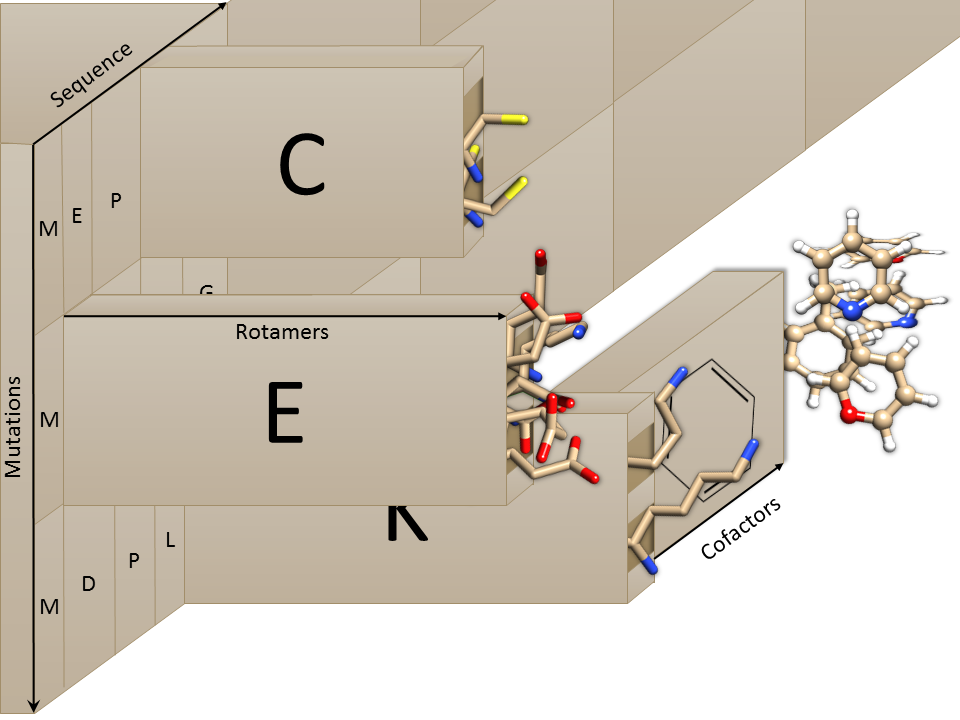
\includegraphics[width=\textwidth]{./figures/02/chemical_space.png}
	\caption[Chemobiological spaces]{
		In any study on protein-ligand interactions, considering sequence mutation of protein scaffolds, each with its possible sidechain orientations, already produces a combinatorial explosion. Taking different possible ligands into account adds one more dimension to the search space. (Reproduced from \textit{Artificial Metalloenzymes and MetalloDNAzymes in Catalysis}\cite{wileybook}).
	}
	\label{fig:chemicalspace}
\end{figure}

\subsubsection{Cheminformatics}
% \addcontentsline{toc}{subsubsection}{Cheminformatics}
There are molecular modeling techniques that do not need to rely on 3D coordinates that information to produce useful results. Cheminformatics are mainly concerned with the creation and maintenance of small compound databases with support for indexation and similarity searches. The main exponent of cheminformatics approaches is probably QSAR techniques.

Quantitative Structure-Activity Relationship (QSAR) studies apply classification or regression statistical techniques to predict experimental observables from basic molecular descriptors. The\ \textit{activity} under study can comprise different variables: biological activity of a drug-like compound, boiling point, potential reactivity, toxicity\ldots\  All QSAR methods are based on the structure-activity relationship (SAR) assumption: similar compounds will have similar activities. The main issue is how to measure that similarity: number of atoms, functional groups, connectivity\ldots\   As in all statistics, large datasets are needed to obtain valid results. The first step in QSAR studies is to train the statistical model with a huge library of compounds. Once the model is trained, it can be used to predict the activity of a compound originally not present in the library.

QSAR input data do not provide 3D-structural data (with the exception of the 3D-QSAR variants), but 2D-topological information. These are normally supplied with special character strings called SMILES (Simplified Molecular Input Line Entry Specification),\cite{smiles} which can describe compounds unambiguously without resorting to explicit coordinates specification. SMILES strings work by enumerating the atoms involved in a molecule with their element symbol, except hydrogen, which is usually implicitly considered. Simple bonds are assumed between linearly adjacent elements. If a ramification occurs, it must be specified with parenthesis. Numeric tags are used to signal the starting and ending atoms of cyclic substructures (see fig. \ref{fig:smiles}). For example, butane would be represented as \texttt{CCCC}, while D-glucose would be \texttt{C(C1C(C(C(C(O1)O)O)O)O)O}.


\begin{figure}[H]
	\begin{center}
	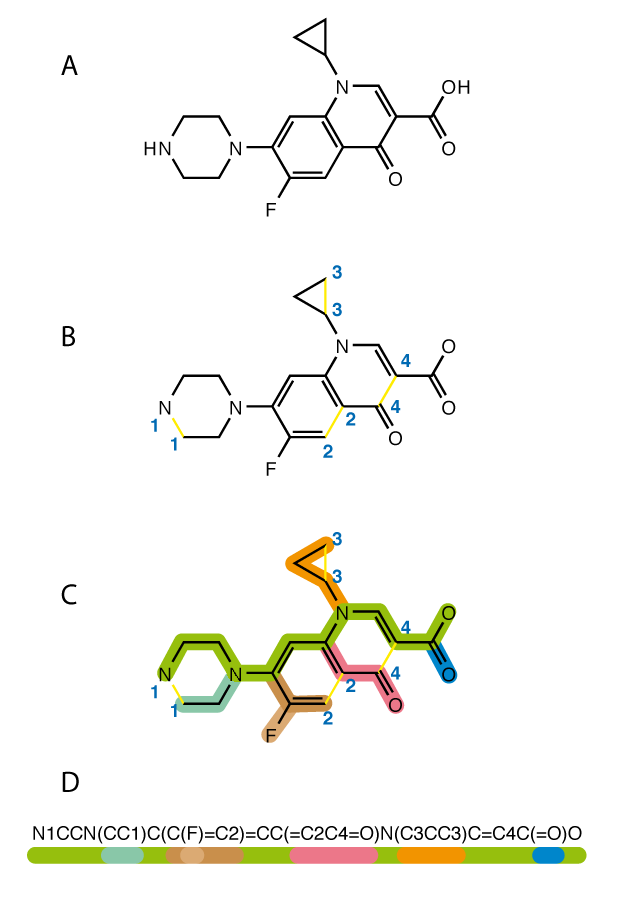
\includegraphics[height=0.9\textheight]{./figures/02/smiles.png}
	\end{center}
	\cprotect\caption[SMILES notation]{SMILES notation can depict a substituted aromatic ring as linear chains with branches. In this case, 3-cyanoanisole is being written as \texttt{COc(c1)cccc1C$\# $N}.}
	\label{fig:smiles}
\end{figure}

\section{Building models from scratch}
\label{section:buildingmodels}
% \addcontentsline{toc}{subsubsection}{Model/topology building}
Up to this point, it has been assumed that the molecular modeler had all the needed input data ready for analysis and simulation, but unfortunately that is not always the case.

In QM studies, when only small molecules are studied, manual building of the model can be contemplated as a possibility using a graphical interface,\cite{gaussview,avogadro} but when the model grows, the possible orientation of rotatable bonds or the configuration of the subunits can be a daunting task to solve manually and even a stopping barrier in the research. Additionally, in some cases, the initial structure is only conceived as a 2D depiction with ChemDraw or similar software, which has to be transformed into a 3D model. This a fairly common process, and as such most software suites include a 2D\textrightarrow 3D converter. However, additional refinements are normally required afterwards. If the system features many degrees of freedom, this can be tedious. A common alternative consists of performing high-temperature molecular dynamics simulations to navigate the conformational landscape. Once the researcher is satisfied, the small compound can be directly minimized with quantum mechanics algorithms, but if the size is too large a short MD simulation might be required instead, in this case to \textit{relax} the structure.

In macromolecular studies where the conformational space is untreatable, experimental data is needed beforehand, like X-Ray Crystallography (XRC) or Nuclear Magnetic Resonance (NMR). These techniques provide density maps to which, with adequate refinement and post-processing using specialized software,\cite{ccp4,phenix} 3D structures are fitted. After validating the quality of the resulting model with ERRAT\cite{errat} or similar protocols, these are then usually submitted to specialized databases like Protein Data Bank (PDB),\cite{proteindatabank} from which the researchers can download the needed files for modeling the required system. Most of the time, files downloaded from PDB must be edited to remove experimental artefacts like duplicate positions of some atoms, protonate the residues at the desired pH by inferring the pKa of each one,\cite{word1999asparagine,propka,addh} or reproduce the biological assembly of the structure.\cite{bietz2016siena,sym}

While the Protein Data Bank holds almost 140,000 structures readily available for everyone, not every protein is there. Sometimes, the structure is partially missing due to experimental limitations or even totally absent. In those cases, the model must be built from scratch. The folding problem is still unsolved and guessing the tertiary structure out of the sequence of amino acids is very challenging, but workarounds exist to work with available data. For example, if the protein that needs to be modeled has an already characterized homolog in the database, their sequence alignment can be used as a template to reconstruct a good structure. This technique is called homology modeling and its accuracy grows when multiple sequence alignment (MSA) are available. Since the final model is only an interpolation of closely related structures, some external validation is needed. In MODELLER, one of the most popular packages for homology modeling, several scoring functions to assess the quality are available. Additionally, a series of web services can be found to help in the task.\cite{errat,benkert2008qmean,wang2011apollo}

Even with a proper protein structure, if the study features custom ligands, obtaining a good candidate for further steps in the protocol is not as simple as one might think. Assuming the required ligand structure is available, a regular protein-ligand docking simulation can provide an initial guess of the complex, but this is usually processed with long MD runs to assess the stability of the interactions. However, if the ligand is not known and must be designed from scratch, there is no consensus strategy. Two common approaches involve: (1) creating a library out of ligands that exhibit the needed chemical features using a reverse pharmacophoric approach, which then would be screened to assess their stability within the protein; (2) applying topology operators during the docking simulation itself using topology operators to dynamically build the ligand out of smaller fragments. The latter has been applied successfully in one the programs presented in this thesis and will be discussed in \autoref{chap:06}.

For larger scale systems like viral capsids or lipid bilayers, which can feature millions of atoms, building a starting structure can be daunting at first, but fortunately they all exhibit some kind of symmetry that can be used to assemble the full structure out of the involved subunits with specialized software.\cite{bietz2016siena,sym}

\section{Optimization methods}

Most of the procedures used to identify physically sound models of a molecular system stand on finding the way to ally the exploration of wide search spaces (like introducing sensible changes in the 3D coordinates of a compound) and the adequate guiding variables (usually, the potential energy). In mathematics, this is territory of optimization problems for non-smooth surfaces.

An optimization problem consists of, given a function $ f $ that connects a set A to ${\rm I\!R}$ finding an element $ x_{0} $ in A such that $ f(x_{0}) \leq f(x) $ for all $ x~in~A $  (minimization), or such that $ f(x_{0}) \geq f(x) $ for all $ x~in~A $ (maximization).

\begin{align}
	Given ~~ f:A \rightarrow R \nonumber \\
	Sought: ~ x_{0} \in A ~ such ~ that ~ f(x_{0})  \leq f(x) ~,~x \in A ~~~ ( minimization ) \nonumber \\
	~~~~~~~~~ or: x_{0} \in A ~ such ~ that ~ f(x_{0})  \geq f(x) ~,~x \in A ~~~ ( maximization )
\end{align}

$ f(x) $  is normally called the objective function, loss function or cost function for minimization problems, utility function or fitness function for maximization problems or, depending on the field, energy function or functional. However, all optimization problems can be expressed as minimization problems, negating  $ f(x) $  if the problem is to be maximized.

The domain  $ A ~ of ~ f $ is usually named the \textit{search space} or the \textit{choice set}, and each possible value of  $ A $  is called a candidate or feasible solution.  $ A $  is normally a subset of  $ R^{n} $ , as defined by equality and/or inequality constraints. The optimization definition can be extended to be subject to inequality and equality constraints, expressed as:

\begin{align}
	optimize_{x}~~~~~~~ f(x) \nonumber \\
	subject~to~~~  g_{i}(x)  \leq 0,~~ i=1,  \ldots ,m \nonumber \\
	~~~~~~~~~~~~~~~~~~~~~~~ h_{j}(x) =0,~~ j=1,  \ldots ,p
\end{align}

, where  \( g_{i}(x)  \)  are the inequality constraints,  \( h_{j}(x)  \)  are the equality constraints, and  \( m \)  and  \( p \)  are greater than 0. If  \( m \)  and  \( p \)  are equal to zero, the definition falls back to the unconstrained optimization problem.

Depending on the form of the function being optimized and the specified constraints, several categories emerge, like convex or nonlinear optimization problems. In convex optimization, $f$, $g$ and $h$ are either convex (minimization) or concave (maximization). This includes linear functions, defining the field of linear optimization. Nonlinear optimization deals with functions that cannot be written as linear expressions, which usually makes the problem harder.

Solving this type of problems was initially studied by Fermat and Lagrange, who applied calculus-based formulae to identify optimum solutions. However, not all optimization problems can be solved analytically and, in fact, for some complex problems is usually easier (and faster) to compute numerical solutions iteratively until a convergence threshold is met. This approach was initiated by Newton and Gauss, and since then many applicable algorithms have been devised throughout the latest decades. A few will be highlighted for illustrative purposes.

\subsection{Steepest descent and conjugate gradient}
% \addcontentsline{toc}{subsubsection}{Steepest descent and conjugate gradient}
To go down a smooth mountain, one simply takes steps in a direction towards the valley. There's a lot of possible directions, but skilled mountaineers usually take the fastest: the steepest side. Climbing down that mountain can be expressed as finding the minimum of a convex three-dimensional function, so figuring out which direction we should take in every step is a matter of finding the gradient of that function at that point.

A gradient is the $n$-dimensional generalization of a single-variable derivative, so instead of returning a scalar, it returns a vector. If derivatives gave us the rate of change of a function, gradients will tell the direction in which the function will experience the greatest change. In this three-dimensional problem, the gradient vector will point to the next step. By taking little steps in the direction pointed by the gradient, we will eventually get to the minimum.

This is what the steepest descent (SD) algorithm does, but it can progress very slowly in almost \textit{flat} regions of the function. A similar method named conjugate gradient (CJ) uses a similar approach, but the search direction is computed in a smarter way, making sure that the direction is orthogonal to the previous step gradient and the current one. It requires more operations, but the performance towards the optimum is better and usually worthy.

Since these methods only compute $f(x)$ and $f’(x)$ (first derivatives), they are called first-order methods.

\subsection{The Newton and quasi-Newton algorithms}
% \addcontentsline{toc}{subsubsection}{The Newton and quasi-Newton algorithms}
Newton numerical algorithms are similar to SD and CJ methods, but compute an additional differentiation step to use the information provided by the curvature of the function. This makes each iteration more expensive, but with certain functions fewer iterations might be needed (see fig. \ref{fig:gradientdescent}).

Second derivatives can be generalized as Hessian matrices for problems of higher dimensions, but this can get very expensive to compute. As a result, several derived methods, called quasi-Newton methods, include alternative methods to compute it or supply equivalent information, like directly computing the inverse with numerical methods, updating it with successive gradient vectors\ldots\ Due to its performance, one of the most popular quasi-Newton algorithms is the BFGS algorithm (for Broyden,\cite{broyden1970convergence} Fletcher,\cite{fletcher1970new} Goldfarb\cite{goldfarb1970family} and Shanno\cite{shanno1970conditioning}) and its limited memory version L-BFGS,\cite{liu1989limited} widely used in energy minimization of molecules.

\begin{figure}[H]
	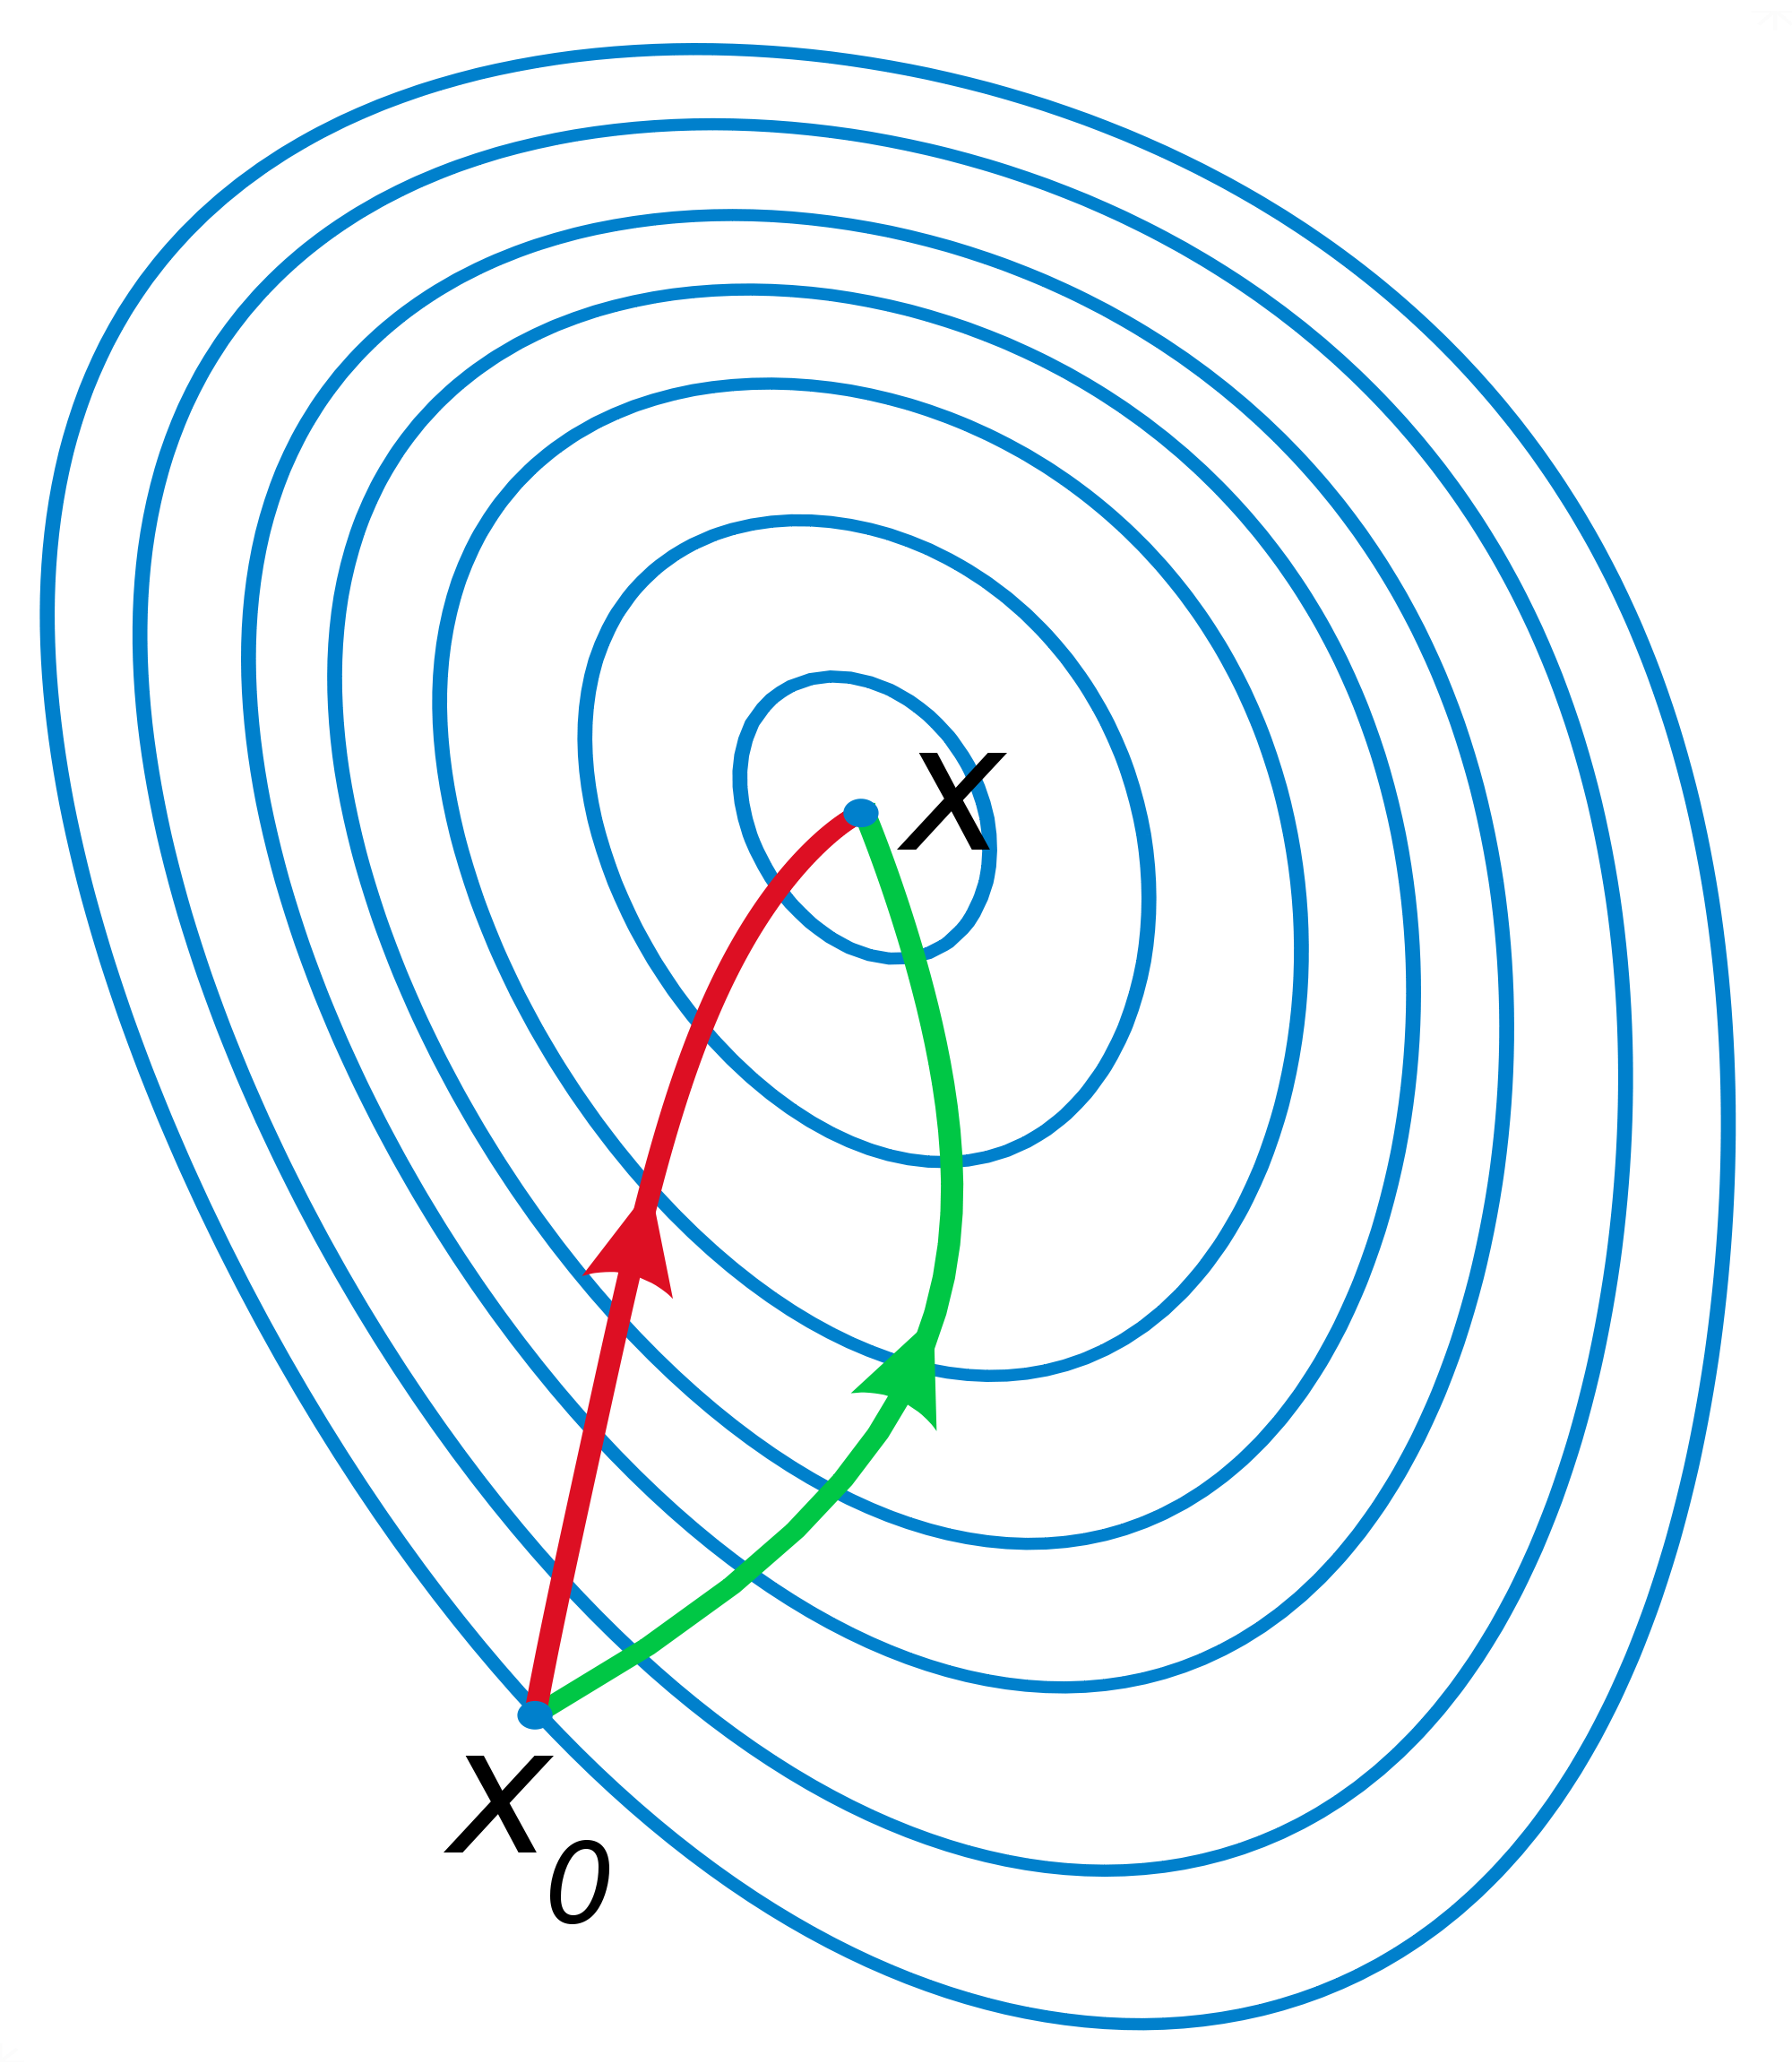
\includegraphics[width=\textwidth]{./figures/04/gradientdescent.png}
	\caption[Gradient descent vs Newton's optimization]{A comparison of gradient descent (green) and Newton's method (red) for minimizing a function (with small step sizes) starting with $ X_{0} $. Global minimum is $ X $. Newton's method uses curvature information to take a more direct route.}
	\label{fig:gradientdescent}
\end{figure}

\subsection{Heuristic and meta-heuristic methods}
% \addcontentsline{toc}{subsection}{Heuristics: thinking abstract but practical}
While all these numerical methods are very different in nature, they still perform the same kind of tasks: exploration, evaluation and selection. This is, they generate a candidate solution (exploration), solve the equations and assess how far they are from the exit condition (evaluation). Selection is often so trivial in scalar functions that is not even considered as a separate step.

In a simplified example, where we must find $f(x) = 0$ with $f(x) = ax + b$, \textit{generating new candidate solutions} would simply consist of assigning new values to $x$. While this can be done randomly until the solution is found, it is usually more interesting to use a smarter approach. This what the gradients and hessian approaches provide: educated guesses towards finding the optima. However, they still require an equation to be available. When several variables are analyzed and the relationship between them is not differentiable or, simply, unknown, other type of algorithms must be employed, like heuristic or meta-heuristic. This kind of methods make very few assumptions about the problem being solved, making them suitable for a variety of optimization areas.

\subsubsection{Monte Carlo methods}
% \addcontentsline{toc}{subsubsection}{Monte Carlo methods}

Monte Carlo methods are useful for studying problems that are characterized by a huge number of degrees of freedom but can be interpreted probabilistically. Since the expected value of an integral can be approximated by the empirical mean of a random sample, these methods allow to obtain numerical results by randomly sampling the search space. In the Metropolis variant, the sample is refined iteratively with random modifications that are either accepted or rejected depending on the new value of the sample or a random acceptance ratio.

For example, to minimize the potential energy of a molecule, random states can be generated by introducing small perturbations to the atomic positions that follow a Boltzmann distribution. The energy of the new states is evaluated and either accepted or rejected by comparing their energies with current mean of the sample. For example, those with smaller energies are usually included and accepted in the ensemble. For those with higher energies, they can still be included with some probability that depends on the chosen acceptance ratio. Being a Markov chain, the probability distribution for the next iteration will be reparameterized with the state of the current sample and the process will continue iteratively until convergence.

\subsubsection{Evolutionary algorithms}
% \addcontentsline{toc}{subsubsection}{Evolutionary algorithms}
Evolutionary algorithms (EA) can be explained as an extension to Monte Carlo's: they also employ random generation of solutions as starting points, but following iterations employ biology-inspired heuristics to localize next candidate solutions. In each iteration, the \textit{population} of feasible solutions (individuals) are evaluated in the optimization environment, and each one is assessed a fitness score. Like in the Evolution theory, only the fittest will be allowed to survive (included in the sample for the next iteration).

Genetic algorithms (GA) are a special type of EA that implement \textit{evolutionary} heuristics inspired on chromosomic changes. By mimicking chromosomes during the meiosis, candidate solutions can exchange some of their variables (mating or recombination), and some can experience a random change in one or more variables (mutation). By iterating over this \textit{reproductive} cycle, fitter and fitter solutions will be obtained.

Besides EA, new metaphor-inspired algorithms are constantly developed. Starting in 1983 with Kirkpatrick's Simulated Annealing (SA),\cite{kirkpatrick1983optimization} it began to grow in the 90s with Ant Colony Optimization\cite{maniezzo1992distributed} and Particle Swarm Optimization,\cite{eberhart1995new} and exploded in the 2000s and 2010s. Last developments have been attracting criticism because they seem to hide the lack of novelty behind an attractive metaphor.\cite{S_rensen_2013,brownlee2015,swan2015research,Glover_2015}

\subsection{Machine learning}
% \addcontentsline{toc}{subsubsection}{Machine learning }
Artificial Intelligence and Machine Learning are very popular computer science fields these days. Globally, they are algorithms that can \textit{learn} from their own \textit{experience} by extracting patterns and relationships out of the supplied data. They can be studied as non-linear statistical data modeling tools.

One of the hottest branches of Machine Learning are Artificial Neural Networks and, especially, Deep Learning. The implemented algorithms in these categories mimic the way neurons work in the brain. Like all mathematical functions, each \textit{neuron} produces an output that depends on the input. Many neurons are grouped together in layers and these layers are concatenated, having the output of one layer fed as the input of the next one. Layers can back-propagate, and modify the input of previous layers, like the feedback mechanism of the brain. Ultimately, this construction generates a huge set of self-adjusting equations that can optimize wide ranges of observations. For example, they are actively used in speech recognition, computer vision or artificial intelligence. The excitement produced by its success in other areas made it permeate towards some areas of science where its application is controversial and less \textit{fancy} algorithms like traditional statistic methods are even better performers.\cite{makridakis2018statistical}

\section{Multi-objective optimization}
\label{section:multiobjective}

Usually, our minds are wired to think in scalar functions and values. This is, functions that return scalar magnitudes or \textit{single values}. If $f(x)$ points to a scalar space, selecting $f(x_{0})$ vs $f(x_{1})$ is just a matter of seeing which value is smaller (minimization) or greater (maximization). However, if the function returns $n$-dimensional data, navigating towards the optimum is not so intuitive. Since there is more than one target value, conflicting decisions might arise.

Say we need to minimize a function that takes a vector in $R^{3}$ and returns another vector in $R^{3}$. Reaching the origin by minimization would mean obtaining a vector with all three values equal to zero. What if the first element in the vector is smaller, but the second is greater? One possibility is to construct a general function out of those functions, like the Euclidean distance until the origin. In more complex cases, simple weighted linear sum might work, but the weights must be carefully chosen for each case; otherwise, convergence problems might appear.\cite{das1997closer}

One alternative which does not involve a dimensionality reduction ($R^{3}$ to $R$ in the previous example) is the Pareto optimality criterion, enunciated by Wilfried F. Pareto in his studies of income distribution in the 1900s. It is based on Pareto \textit{dominance}: a solution $a$ is set to dominate solution $b$ if it solves at least one of the objectives better than $b$, without losing to $b$ in any of the remaining objectives.\cite{deb1999multi} By enumerating a high number of solutions and comparing them in terms of Pareto-dominance, a reduced set of non-dominated solutions can be found (see fig. \ref{fig:pareto}). When no more non-dominated solutions can be found, that set is said to be Pareto-optimal and constitutes the Pareto front: the solutions to the problem.\footnote{Optimization processes like this are more common that they appear. At the supermarket, all clients decide on the trade-off between price and quality every day. Normally, humans solve this by setting a cutoff on one of the variables. For example, a maximum budget is set. However, if all possibilities are considered, the resulting solutions would range from the cheapest possible product to the most expensive one, including all the good enough (non-dominated) combinations in between. However, if a new product is added to the catalog and is cheaper than its competitors without a decrease in quality, that new product will dominate all other products with the same quality but higher price.}

Under this scheme, finding the solutions to a multi-objective problem is only a matter of increasingly enriching the Pareto front with non-dominated solutions. Without defining the importance of each objective, all of them will be equally good solutions. In other words, multi-objective optimization algorithms do not propose a single optimum solution, but a set of good trade-offs between the variables under consideration.\cite{coello2007evolutionary}


\begin{figure}[H]
	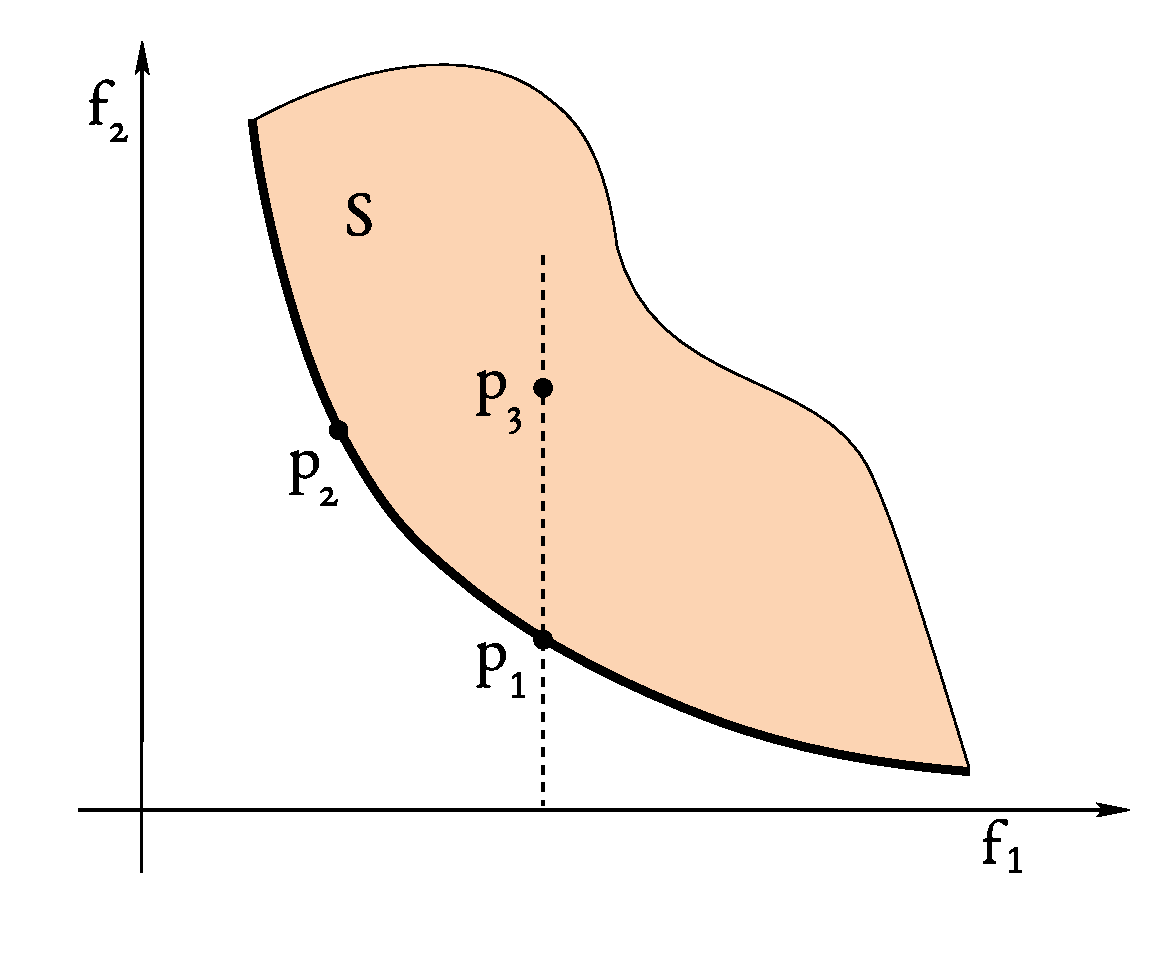
\includegraphics[width=\textwidth]{./figures/02/FrentePareto.pdf}
	\caption[A Pareto front for two dimensions]{For a two-dimensional problem where $f_{1}$ and $f_{2}$ must be minimized, the Pareto front can be identified with a convex curve. In this example, $p_{1}$ and $p_{2}$ are non-dominated solutions that are part of the Pareto front (wide line). $p_{3}$ is dominated by $p_{1}$ and $p_{2}$ because $p_{1}$ has a lower value in the $f_{2}$ axis without worsening the value in the $f_{1}$ axis, and $p_{2}$ has lower values in both axes.}
	\label{fig:pareto}
\end{figure}

% \section{Python programming}

% \todo[inline]{Do we really needa a Python section here?}

% - High-level expressivity
% - Availability of packages
% - Intuitive syntax
% - Sane community
% - Problems: packaging, performance?